\documentclass[]{article}

% Get better typography
\usepackage[protrusion=true,expansion=true]{microtype}		

% For algorithms
\usepackage[boxruled,linesnumbered,vlined,inoutnumbered]{algorithm2e}
\SetKwInOut{Parameter}{Parameters}

% For basic math, align, fonts, etc.
\usepackage{amsmath}
\usepackage{amssymb}
\usepackage{mathtools}
\usepackage{mathrsfs}
\usepackage{enumitem}

\DeclareMathOperator*{\argmin}{arg\,min}
\DeclareMathOperator*{\argmax}{arg\,max}

% For color
\usepackage{xcolor}
\definecolor{light-grey}{rgb}{0.9,0.9,0.9}
\definecolor{dark-red}{rgb}{0.4,0.15,0.15}
\definecolor{dark-blue}{rgb}{0,0,0.7}

% For links (e.g., clicking a reference takes you to the phy)
\usepackage{hyperref}
\hypersetup{
    colorlinks, linkcolor={dark-blue},
    citecolor={dark-blue}, urlcolor={dark-blue}
}

%-------------------------
%	BEGIN DOCUMENT / TITLE
%-------------------------
\begin{document}
\begin{center}
    \begin{Large}
    CMPSCI 687 Homework 4
    \end{Large}
    \\
    Due November 14, 2019, 11:55pm Eastern Time
\end{center}
\addcontentsline{toc}{subsection}{\textbf{Homework 4}}

\noindent {\bf Instructions: } Collaboration is not allowed on any part of this assignment. Submissions must be typed (hand written and scanned submissions will not be accepted). You must use \LaTeX. The assignment should be submitted as five documents: a .pdf with your written answers, two .hpp files, and two .cpp files as described in the programming portion.
\\\\
\section*{Programming (75 Points Total)}

In this assignment, you will implement Sarsa and $Q$-learning, and will apply them to a gridworld (not the one from the course notes), mountain car, acrobot, and cart-pole. Begin with the source code provided \href{https://people.cs.umass.edu/~pthomas/courses/CMPSCI_687_Fall2019/HW4Source.zip}{here} (see the previous assignments for instructions regarding opening the project). Look at main.cpp, starting with the function main. Look through how this code functions: it applies Sarsa and Q-learning to various MDPs in sequence. Hyperparameters (not good ones!) are specified for each environment in main.cpp.\footnote{For this assignment, you may view the iOrder and dOrder hyperparameters as both being the order of the Fourier basis, and you may always set them to the same value.} The code for Sarsa should be in Sarsa.hpp (a header file, that defines the Sarsa class) and Sarsa.cpp (the source file, that includes the actual code for all of the functions that a Sarsa object requires). Similarly the code for Q-learning is split across QLearning.hpp and QLearning.cpp. You should fill code into Sarsa.hpp, Sarsa.cpp, QLearning.hpp, and QLearning.cpp, and these four files are the four that you should submit with your assignment.

To be clear, your edits should be: 1) changing the hyperparameters specified in main.cpp (you do not have to submit these, but will report hyper-parameter values in your write-up), 2) adding code to the train function in QLearning.cpp (you may change QLearning.hpp and other functions in QLearning.cpp, but this is not necessary), 3) adding code to Sarsa.hpp (private member variables) and Sarsa.cpp (likely all of the functions except for ``getAction'' will have code that you add).

After reading through main.cpp to see what it does, look through Gridworld.hpp and Gridworld.cpp. Gridworld.hpp and Gridworld.cpp have been commented more heavily than the files for the other MDPs. These provide an example of a class in C++. The .hpp file contains the definition of the Gridworld object, and the .cpp file implements the functions that it requires. This also shows how the environments all work. Notice, for example, that the getState() function normalizes the state for you -- it returns the state as a vector, each element of which is in the interval $[0,1]$. Notice also that this code is set up to work well with linear function approximation, as the state is a vector of floating point numbers (not yet features!) that can be provided to the FourierBasis class to convert to features.

Now that you've read through main.cpp and Gridworld.cpp, look at QLearning.hpp and QLearning.cpp. QLearning.hpp and QLearning.cpp have been commented more heavily than the files for Sarsa. Most of this class is implemented for you. The ``train'' function has not been implemented fully -- you must fill this in. Notice some useful functions have been provided in MathUtils.hpp, like ``dot''. Also, note that this time we are not using the Eigen library. Don't be afraid to use for loops though, as these are very efficient in C++. The computational bottleneck in this code is usually computing the cosines in the FourierBasis object. This is why we compute and store the features for state $s'$ in an $(s,a,r,s')$ tuple, so that we can re-use them at the next iteration for state $s$. We could be even more efficient by not recomputing features whenever the agent is asked for an action (right now, QLearning will compute features for state $s$ twice, once in the train function and once in the getAction function). For this assignment, this inefficiency is ok.

Once you have implemented the train function in QLearning.cpp, try setting the hyperparemeters in main.cpp to get results similar to those in the provided file ``plots.xlsx''. If, after running your code, you copy the contents of the other .csv files over the entries in plots.xlsx, it should update to show the plots we want. You are welcome to use your own system (e.g., write your own python code) to make plots from the output .xlsx files. Hint: For both Q-Learning and Sarsa, set $q(s',a')=0$ when computing the TD-error if $s'$ is a terminal state, since we know this action-value and therefore do not need to approximate it.

Next, look at Sarsa.hpp and Sarsa.cpp. These are left more empty for you to fill in. Importantly, we're making this harder for you that just putting in the pseudocode. Look back at Section 3.1. The pseudocode there works well for Q-learning, but not as well for Sarsa, since Sarsa requires the action $a'$ to update. Notice that main.cpp implements the pseudocode from Section 3.1. So, you must write Sarsa in a way that works with this setup. Hint: you will want the agent to have some memory, perhaps remembering which states, actions, and/or rewards it saw previously.

Point allocations for this assignment will be determined at the time of grading, based on which mistakes and issues are common.

\begin{enumerate}
    \item Describe the process of implementing Q-Learning. Did everything work immediately? Did you have bugs that you had to fix? What were they?
    \\\\
    \textcolor{blue}{
		To implement Q-learning, I had to implement the TD update by calculating the TDError in the train method using the following formulation:\\
		$\delta = r - gamma*\max_{a \in \mathcal{A}}(q(s',a')) + q(s,a)$\\
		$\max_{a \in \mathcal{A}}(q(s',a')) = maxQ(\phi(s'))$ \\
		$q(s,a) = w[a] . \phi(s)$\\
		I then updated the weight for action $a$ as follows:\\
		$w[a][i] += \alpha*\delta*\phi[i]$ $\forall i $\\
		I was able to get everything working immediately and there were no bugs in the code.
	}

    \item Describe the process of implementing Sarsa. Did everything work immediately? Did you have bugs that you had to fix? What were they?
    \\\\
    \textcolor{blue}{
    	Implementation of Sarsa was more nuanced. The TD Error required both $a$ and $a'$ but sampling $a'$ inside the train method lead to mismatch in the action used during the update and the action used to interact with the environment in the runExperiment method which would sample the action again. I kept a variable to track the previous action ($prevAction$), previous reward ($prevR$)as well as the previous value of $\phi(s)$ ($prevPhi$) and updated the weights for the action in the subsequent call to train. I had to skip this update in the very first call to train. I also had to handle the case of $s'$ being terminal separately in order to additionally update the weights for action $a$. Updates were made using the following formulation:\\
    	$\delta = r - gamma*q(s,a) + q(prevState,prevAction)$\\
    	$q(s,a) = w[a].\phi(s) = w[a].phi $\\
    	$q(prevState,prevAction) = w[prevAction] . prevPhi$\\
    	I then updated the weight for action $prevAction$ as follows:\\
    	$w[prevAction][i] += \alpha*\delta*prevPhi[i]$ $\forall i $\\
    	Additionally, when $s'$ was terminal, the following update would also be made for action $a$:\\
    	$w[a][i] += \alpha*\delta*phi[i]$ $\forall i $\\
       	I was able to get everything working immediately and there were no bugs in the code.
    }

    \item Describe the process of optimizing the hyperparameters for Q-Learning for MountainCar, and report the final hyperparameters that you found.
    \\\\
    \textcolor{blue}{
    	The final hyperparameters found were :\\
    	$
    	\alpha  = 0.005,
    	\gamma = 0.99,
    	\epsilon = 0.1,
    	iOrder = 3,
    	dOrder = 2
    	$\\
    	I started with $dOrder$ of 2 as I had used a $2^{nd}$ order Fourier basis for the BBO implementations in the earlier homework. I searched for values of $\epsilon$ in the range of $0.1$ to $0.001$ and values of $\alpha$ in the range of $1$ to $0.001$.  I started with small values for both and then gradually them. Increasing $\epsilon$ improved the learning but the increasing $\alpha$ seemed to cause divergence where the algorithm would suddenly stop learning and returns would go down. I then kept the value of $\alpha$ small and increased $\epsilon$ till the algorithm converged. I tried a few values of $\gamma$ ranging from $0.9$ to $0.999$ and found that $0.99$ worked well.
    }

    \item Describe the process of optimizing the hyperparameters for Q-Learning for CartPole, and report the final hyperparameters that you found.
    \\\\
    \textcolor{blue}{
    	The final hyperparameters found were :\\
    	$
    	\alpha  = 0.01,
    	\gamma = 0.9,
    	\epsilon = 0.05,
    	iOrder = 3,
    	dOrder = 2
    	$\\
    	I started with $iOrder$ of 2 as I had used a $2^{nd}$ order Fourier basis for the BBO implementations in the earlier homework. I searched for values of $\epsilon$ in the range of $0.1$ to $0.001$ and values of $\alpha$ in the range of $1$ to $0.001$.  I started with small values for both and then gradually increased $\epsilon$ till the algorithm converged without having to increase $\alpha$. Increasing $\epsilon$ also increased the standard deviation in the result. Increasing $\epsilon$ increased the standard deviation in the result. I tried a few values of $\gamma$ ranging from $0.9$ to $0.999$ and found that $0.9$ worked well.
    }

    \item Describe the process of optimizing the hyperparameters for Q-Learning for Acrobot, and report the final hyperparameters that you found.
    \\\\
    \textcolor{blue}{
    	The final hyperparameters found were :\\
    	$
    	\alpha  = 0.001,
    	\gamma = 0.99,
    	\epsilon = 0.1,
    	iOrder = 4,
    	dOrder = 3
    	$\\
    	Acrobot required a substantially higher order represtation. I searched for values of $\epsilon$ in the range of $0.1$ to $0.001$ and found the lower values worked better. I searched for values of $\alpha$ in the range of $1$ to $0.001$. I started with a high value of $\alpha$ and a low value of $\epsilon$ but the algorithm did not converge. I then started reducing the alpha and increasing $\epsilon$ to add more randomness to the process. Increasing $\epsilon$ increased the standard deviation in the result. I tried a few values of $\gamma$ ranging from $0.9$ to $0.999$ and found that $0.99$ worked well.
    }

    \item Describe the process of optimizing the hyperparameters for Q-Learning for Gridworld, and report the final hyperparameters that you found.
    \\\\
    \textcolor{blue}{
    	The final hyperparameters found were :\\
    	$
    	\alpha  = 0.05,
    	\gamma = 0.99,
    	\epsilon = 0.001,
    	iOrder = 1,
    	dOrder = 0
    	$\\
    	As suggested, I did not change iOrder and dOrder to keep a tabular representation. I searched for values of $\epsilon$ in the range of $0.1$ to $0.001$ and found that lower values worked better. I searched for values of $\alpha$ in the range of $1$ to $0.001$ with very high values resulted in some quick high return values but then fell off and did not converge whereas very low values did not seem to learn fast enough and stayed at low return values. I tried a few values of $\gamma$ ranging from $0.9$ to $0.999$ and found that $0.99$ worked well.
    }


    \item Describe the process of optimizing the hyperparameters for Sarsa for MountainCar, and report the final hyperparameters that you found.
    \\\\
    \textcolor{blue}{
    	The final hyperparameters found were :\\
    	$
    	\alpha  = 0.005,
    	\gamma = 0.99,
    	\epsilon = 0.1,
    	iOrder = 3,
    	dOrder = 2
    	$\\
    	I started with $iOrder$ of 2 as I had used a $2^{nd}$ order Fourier basis for the BBO implementations in the earlier homework. I searched for values of $\epsilon$ in the range of $0.1$ to $0.001$ and values of $\alpha$ in the range of $1$ to $0.001$.  I started with small values for both and then gradually them. Increasing $\epsilon$ improved the learning but the increasing $\alpha$ seemed to cause divergence where the algorithm would suddenly stop learning and returns would go down. I then kept the value of $\alpha$ small and increased $\epsilon$ till the algorithm converged. I tried a few values of $\gamma$ ranging from $0.9$ to $0.999$ and found that $0.99$ worked well. Surprisingly, the same values of hyperparameters that worked for Q-learning also worked for Sarsa.
    }

    \item Describe the process of optimizing the hyperparameters for Sarsa for CartPole, and report the final hyperparameters that you found.
    \\\\
    \textcolor{blue}{
    	The final hyperparameters found were :\\
    	$
    	\alpha  = 0.01,
    	\gamma = 0.99,
    	\epsilon = 0.1,
    	iOrder = 3,
    	dOrder = 2
    	$\\
    	I started with $dOrder$ of w as I had used a $2^{nd}$ order Fourier basis for the BBO implementations in the earlier homework. I searched for values of $\epsilon$ in the range of $0.1$ to $0.001$ and values of $\alpha$ in the range of $1$ to $0.001$.  I started with small values for both and then gradually increased $\epsilon$ till the algorithm converged without having to increase $\alpha$. Increasing $\epsilon$ also increased the standard deviation in the result. Sarsa required a higher randomness factor than Q-learning. Increasing $\epsilon$ increased the standard deviation in the result. I tried a few values of $\gamma$ ranging from $0.9$ to $0.999$ and found that $0.99$ worked well.
    }

    \item Describe the process of optimizing the hyperparameters for Sarsa for Acrobot, and report the final hyperparameters that you found.
    \\\\
    \textcolor{blue}{
    	The final hyperparameters found were :\\
    	$
    	\alpha  = 0.001,
    	\gamma = 0.99,
    	\epsilon = 0.01,
    	iOrder = 4,
    	dOrder = 3
    	$\\
    	Acrobot required a substantially higher order represtation. I searched for values of $\epsilon$ in the range of $0.1$ to $0.001$ and values of $\alpha$ in the range of $1$ to $0.001$. I started with a high value of $\alpha$ and a low value of $\epsilon$ but the algorithm did not converge. I then started reducing the alpha and increasing $\epsilon$ to add more randomness to the process. Sarsa was able to converge with a smaller value of $\epsilon$ than Q-learning. Increasing $\epsilon$ increased the standard deviation in the result. I tried a few values of $\gamma$ ranging from $0.9$ to $0.999$ and found that $0.99$ worked well.
    }

    \item Describe the process of optimizing the hyperparameters for Sarsa for Gridworld, and report the final hyperparameters that you found.
    \\\\
    \textcolor{blue}{
    	The final hyperparameters found were :\\
    	$
    		\alpha  = 0.05,
    		\gamma = 0.99,
    		\epsilon = 0.001,
    		iOrder = 1,
    		dOrder = 0
    	$\\
    	As suggested, I did not change iOrder and dOrder to keep a tabular representation. I searched for values of $\epsilon$ in the range of $0.1$ to $0.001$ and found that lower values worked better. I searched for values of $\alpha$ in the range of $1$ to $0.001$ with very high values resulted in some quick high return values but then fell off and did not converge whereas very low values did not seem to learn fast enough and stayed at low return values. I tried a few values of $\gamma$ ranging from $0.9$ to $0.999$ and found that $0.99$ worked well. Surprisingly, the same hyperparameters that worked for Q-learning also worked for Sarsa.
    }
    
    \item Provide four plots, one per environment, showing the learning curves for Sarsa and Q-learning with the best hyperparameters that you found. Keep the number of trials, number of episodes, and maxEpisodeLength terms from the provided main.cpp. Include error bars showing one standard deviation. These plots can be created using any plotting software of your choice.
    
    \begin{figure}[h!]
    	\hspace*{0.1\textwidth}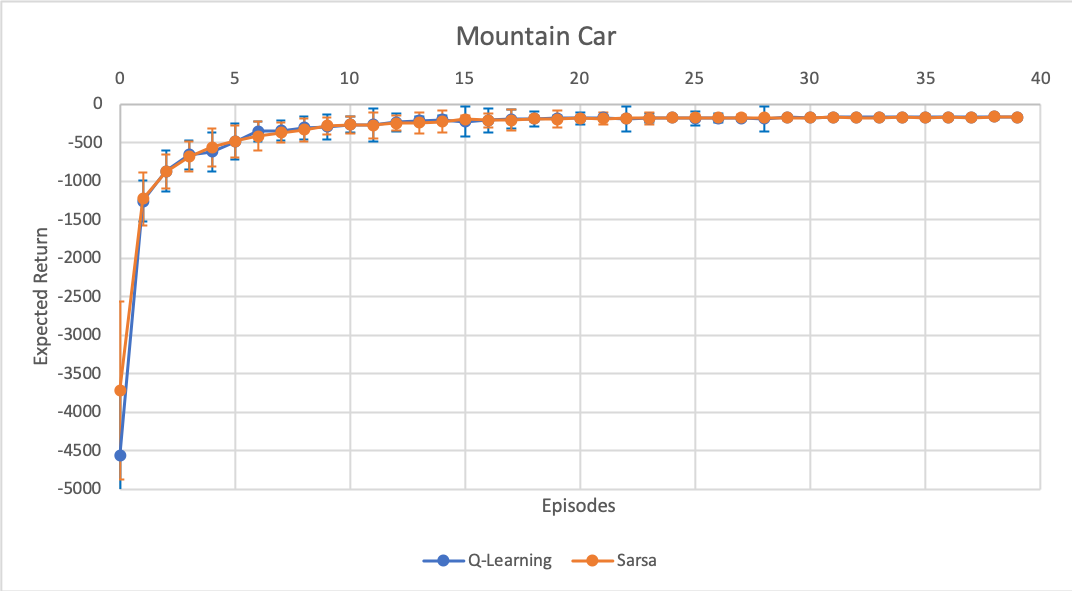
\includegraphics[width=0.8\textwidth]{MountainCar.png}
    	\label{fig: Learning Curve - Mountain Car}
	\end{figure}
	\begin{figure}
		\hspace*{0.1\textwidth}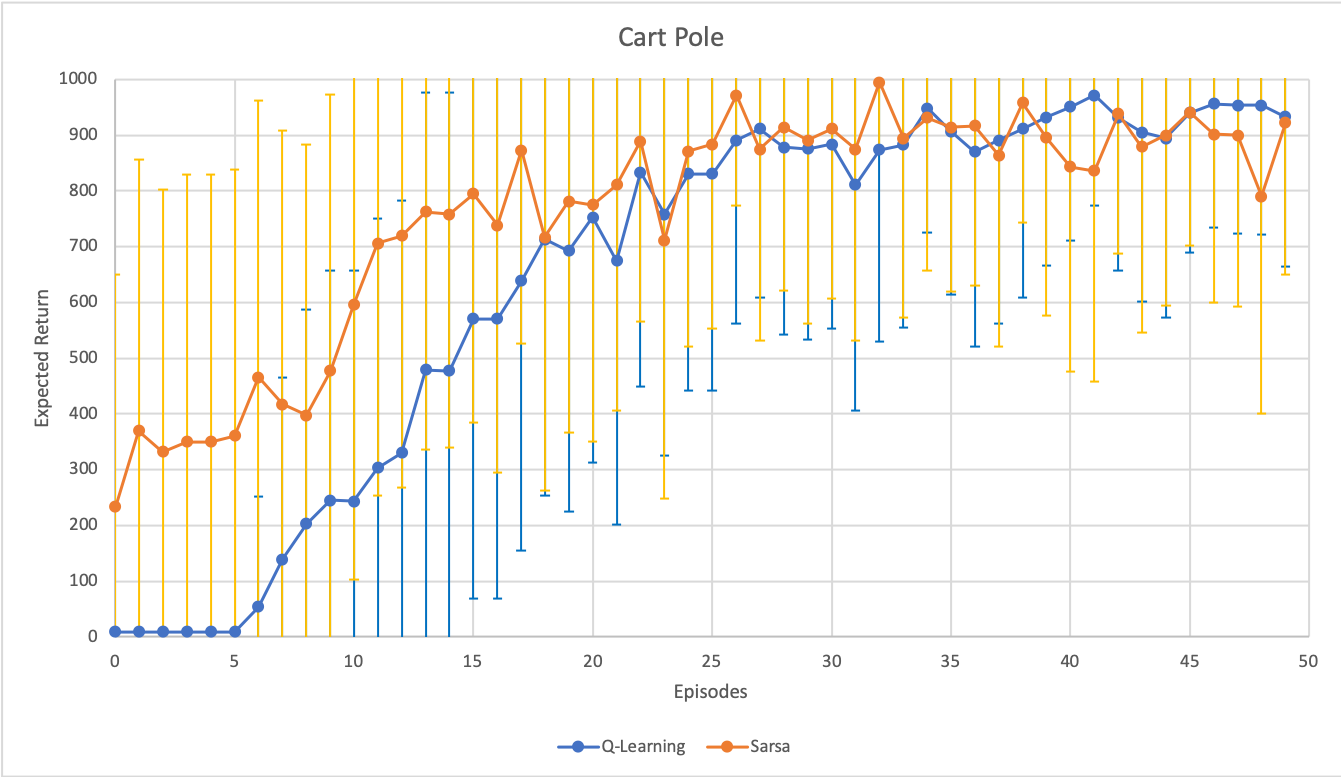
\includegraphics[width=0.8\textwidth, ]{CartPole.png}
		\label{fig: Learning Curve - CartPole}
	\end{figure}
	\begin{figure}
		\hspace*{0.1\textwidth}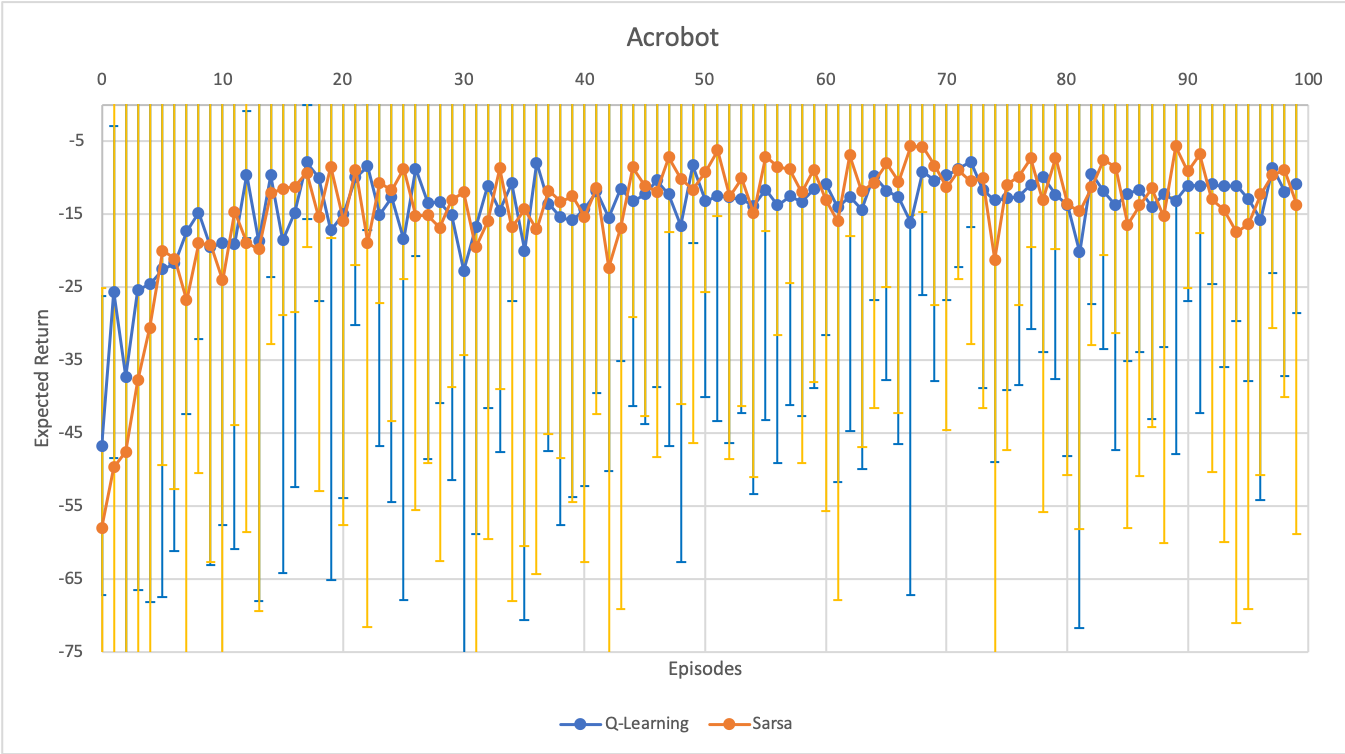
\includegraphics[width=0.8\textwidth]{Acrobot.png}
		\label{fig: Learning Curve - Acrobot}
	\end{figure}
	\begin{figure}
		\hspace*{0.1\textwidth}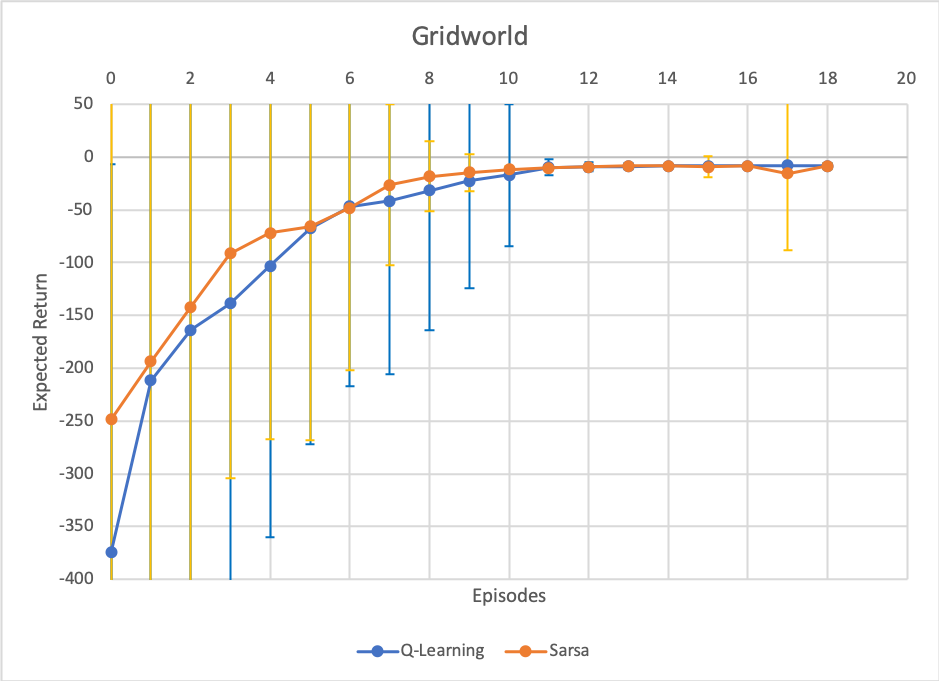
\includegraphics[width=0.8\textwidth]{Gridworld.png}
		\label{fig: Learning Curve - Gridworld}
	\end{figure}
    \pagebreak
    \item Compare your experiences with Q-Learning and Sarsa to your experiences with BBO. Which did you find easier to get working? Which algorithms learned fastest on Cart-Pole (in HW2, you implemented BBO algorithms for Cart-Pole)?
    \\\\
	\textcolor{blue}{
		Answer:\\
		Q-learning and Sarsa were much easier to train and converged remarkably faster than BBO algorithms. BBO algorithms took several thousand episodes to converge while Sarsa just takes about 30 and Q-learning about 40 to converge on the Cart-Pole domain. Sarsa and Q-learning learned the fastest with Q-learning converging slightly slower than Sarsa but to a better policy. Sarsa seemed more sensitive to the hyperparameters than Q-learning.
	}

    \item Be sure to submit your QLearning.hpp (even if it is unchanged, as recommended), QLearning.cpp, Sarsa.hpp, and Sarsa.cpp files with your write-up.
    \textcolor{blue}{Submitted}
\end{enumerate}

Note: This code is written to be relatively simple, as many of you are new to C++. This does not represent best coding practices (e.g., we could make use of subclasses).

\end{document}
